\documentclass[12pt,A4paper]{article}
%\pdfoutput=1

\usepackage{multirow}
\usepackage{cite}
\usepackage{hyperref}
\usepackage{slashed}
\usepackage{graphicx}
    \usepackage{amsmath}
    \usepackage{caption}
    \usepackage{subcaption}
    \usepackage{cancel}
    \usepackage{etoolbox} % provides \patchcmd macro
    \makeatletter % modify the "headings" page style
    \patchcmd{\ps@headings}{{\slshape
ightmark}\hfil	hepage}{	hepage\hfil}{}{}
    \makeatother
    \pagestyle{headings}
\usepackage{listings}
\usepackage{color}
\usepackage{appendix}

\textwidth 170mm
\textheight 220mm
\oddsidemargin -5mm
\evensidemargin 5mm
\topmargin -16pt

\newcommand{\colspacea}{\hphantom{33333333}}
\newcommand{\colspaceb}{\hphantom{33333333}}
\newcommand{\colspacec}{\hphantom{33333333}}
\newcommand{\colspace}{\hphantom{33333333333}}


\newcommand{\xspace}{~}
\newcommand{\GeV}{\ensuremath{\,\text{Ge\hspace{-.08em}V}}\xspace}
\newcommand{\PSGczDo}{\ensuremath{\widetilde{\chi}^{0}_{1}}\xspace} % neutralino
\newcommand{\Pp}{\ensuremath{p}}
\newcommand{\PSg}{\ensuremath{\widetilde{g}}}
\newcommand{\PQq}{\ensuremath{q}}
\newcommand{\cPqt}{\ensuremath{t}}
\newcommand{\cPq}{\ensuremath{q}}
\newcommand{\cPqb}{\ensuremath{b}}
\newcommand{\PAQq}{\overline{\ensuremath{q}}}
\newcommand{\cPaqt}{\overline{\ensuremath{t}}}
\newcommand{\cPaqb}{\overline{\ensuremath{b}}}
\newcommand{\PSQ}{\ensuremath{\widetilde{q}}}
\newcommand{\PSGcz}{\ensuremath{\widetilde{\chi_0^1}}}
\newcommand{\qqbar}{\ensuremath{\PQq\PAQq}\xspace}
%\newcommand{\mgluino}{\ensuremath{m_{\PSg}}\xspace}
\newcommand{\HT}{\ensuremath{H_{\mathrm T}}\xspace}
\newcommand{\MHT}{\ensuremath{H_{\mathrm T}^{\text{miss}}}\xspace}
\newcommand{\njets}{\ensuremath{N_{\text{jet}}}~}
\newcommand{\nbjets}{\ensuremath{N_{\text{b-jet}}}~}
\newcommand{\mgluino}{\ensuremath{m_{\PSg}}\xspace}
\newcommand{\msquark}{\ensuremath{m_{\PSQ}}\xspace}
%\newcommand{\mlsp}{\ensuremath{m_{{\PSGcz}_1}}\xspace}
\newcommand{\tbbar}{\ensuremath{\cPqt\cPaqb}\xspace} % t-bbar
\newcommand{\ttbar}{\ensuremath{t\overline{t}}\xspace} % t-tbar
\newcommand{\bbbar}{\ensuremath{b\overline{b}}\xspace} % b-bbar
\newcommand{\sTop}{\ensuremath{\widetilde{t}}\xspace}
\newcommand{\sBot}{\ensuremath{\widetilde{b}}\xspace}
\newcommand{\sQua}{\ensuremath{\widetilde{q}}\xspace}
\newcommand{\PASQt}{\ensuremath{\overline{\widetilde{t}}}\xspace} % anti stop
\newcommand{\PASQb}{\ensuremath{\overline{\widetilde{b}}}\xspace} % anti sbottom
\newcommand{\PASQ}{\ensuremath{\overline{\widetilde{q}}}\xspace} % anti squark




\newcommand{\neles}{\ensuremath{N_{\text{electron}}}\xspace}
\newcommand{\nmuons}{\ensuremath{N_{\text{muon}}}\xspace}
\newcommand{\nisomuons}{\ensuremath{N_{\text{isolated tracks}}^{\text{(muon)}}}\xspace}
\newcommand{\nisoeles}{\ensuremath{N_{\text{isolated tracks}}^{\text{(electron)}}}\xspace}
\newcommand{\nisohads}{\ensuremath{N_{\text{isolated tracks}}^{\text{(hadron)}}}\xspace}
\newcommand{\dpmht}[1]{\ensuremath{\Delta\phi_{\MHT,j_{#1}}}\xspace}


\newcommand{\mulobs}{$\sigma^{\mathrm{UL}}_{\mathrm{obs}}$}
\newcommand{\ulobs}{\sigma^{\mathrm{UL}}_{\mathrm{obs}}}
\newcommand{\mulexp}{$\sigma^{\mathrm{UL}}_{\mathrm{exp}}$}
\newcommand{\ulexp}{\sigma^{\mathrm{UL}}_{\mathrm{exp}}}
\newcommand{\mtheo}{$\sigma^{\mathrm{pred}}_{\mathrm{theo}}$}
\newcommand{\theo}{\sigma_{\mathrm{pred}}^{\mathrm{theo}}}

\newcommand{\lumi}{\mathcal{L}}
\newcommand{\twomm}{\hspace{2mm}}
\newcommand{\neu}{{\widetilde{\chi}_1^0}}

\newcommand{\go}{{\widetilde{g}}}
\newcommand{\sq}{{\widetilde{q}}}
\newcommand{\mmsq}{$m_{\widetilde{q}}$}
\newcommand{\msq}{m_{\widetilde{q}}}
\newcommand{\mlsp}{m_{\widetilde{\chi}}}
\newcommand{\mmlsp}{$m_{\widetilde{\chi}}$}
\newcommand{\mgo}{m_{\widetilde{g}}}
\newcommand{\mmgo}{$m_{\widetilde{g}}$}

\definecolor{dkgreen}{rgb}{0,0.6,0}
\definecolor{gray}{rgb}{0.5,0.5,0.5}
\definecolor{mauve}{rgb}{0.58,0,0.82}
\lstset{ %
  language=C++,                % the language of the code
  basicstyle=\footnotesize,           % the size of the fonts that are used for the code
  %  numbers=left,                   % where to put the line-numbers
  %  numberstyle=\tiny\color{gray},  % the style that is used for the line-numbers
  %  stepnumber=2,                   % the step between two line-numbers. If it's 1, each line
  % will be numbered
  %  numbersep=5pt,                  % how far the line-numbers are from the code
  backgroundcolor=\color{white},      % choose the background color. You must add \usepackage{color}
  showspaces=false,               % show spaces adding particular underscores
  showstringspaces=false,         % underline spaces within strings
  showtabs=false,                 % show tabs within strings adding particular underscores
  frame=single,                   % adds a frame around the code
  rulecolor=\color{black},        % if not set, the frame-color may be changed on line-breaks within not-black text (e.g. commens (green here))
  tabsize=2,                      % sets default tabsize to 2 spaces
  captionpos=b,                   % sets the caption-position to bottom
  breaklines=true,                % sets automatic line breaking
  breakatwhitespace=false,        % sets if automatic breaks should only happen at whitespace
  title=\lstname,                   % show the filename of files included with \lstinputlisting;
  % also try caption instead of title
  keywordstyle=\color{blue},          % keyword style
  commentstyle=\color{dkgreen},       % comment style
  stringstyle=\color{mauve},         % string literal style
  escapeinside={\%*}{*)},            % if you want to add a comment within your code
  morekeywords={*,\dots}               % if you want to add more keywords to the set
}


\title{Validation of the \texttt{MadAnalysis 5} implementation of CMS-EXO-16-012}
\author{Jiwon Park, Seohyun Ahn (Hanyang Unibversity) \and Wenxing Zhang (ITP of Chinese Academy of Science)\\
\normalsize {\it email: jiwon.park@cern.ch}
\date{\today}
}

\begin{document}
        \maketitle

%\clearpage
%%%%%%%%%%%%%%%%%%%%%%%%%%%%%%%%%%%%%%%%%%%%%%%%%
%%%%%%%%%%%%%%%    Setup   %%%%%%%%%%%%%%%%%%%%%%
%%%%%%%%%%%%%%%%%%%%%%%%%%%%%%%%%%%%%%%%%%%%%%%%%

\section{Setup}
\indent In this document, the \texttt{MadAnalysis 5} implementation of search for associated production of dark matter with a
Higgs boson decaying to \bbbar or $\gamma\gamma$ at $\sqrt{s} = 13$ TeV (2.3 fb$^{-1}$),
\href{http://cms-results.web.cern.ch/cms-results/public-results/publications/EXO-16-012/}
(see also \href{https://arxiv.org/abs/1703.05236}{arXiv:1703.05236})
is validated.

For this purpose, model UFO, MG5 cards, and a pythia8 card for Monte Carlo production were provided by CMS to generate events with \texttt{MadGraph MG5\_aMC}, showered with \texttt{Pythia 8}

This paper is written in the context of $Z'$-two-Higgs-doublet model, where a high-mass resonance $Z'$ decays into a pseudoscalar boson $A$ and a CP-even scalar Higgs boson, and the A decays to a pair of dark matter particles.

To generate signal sample, \href{http://rkhurana.web.cern.ch/rkhurana/monoH/models/}{model UFO files} is provided by CMS. From the \href{https://github.com/cms-sw/genproductions/tree/master/bin/MadGraph5_aMCatNLO/cards/production/13TeV/monoHiggs/Zp2HDM/Zprime_A0h_A0chichi}{CMS genproduction gitbub repository} one can retrieve the cards used for \texttt{MadGraph MG5\_aMC} event generation for each mass point of $Z'$. 
The \href{https://github.com/cms-sw/genproductions/blob/master/bin/MadGraph5_aMCatNLO/cards/production/13TeV/monoHiggs/Zp2HDM/Zprime_A0h_A0chichi/Zprime_A0h_A0chichi_MZp600_MA0300/Zprime_A0h_A0chichi_MZp600_MA0300_run_card.dat}{run card} used in \texttt{MadGraph MG5\_aMC} and \href{https://github.com/cms-sw/genproductions/blob/master/bin/MadGraph5_aMCatNLO/cards/production/13TeV/monoHiggs/Zp2HDM/Zprime_A0h_A0chichi/Zprime_A0h_A0chichi_MZp600_MA0300/Zprime_A0h_A0chichi_MZp600_MA0300_proc_card.dat}{proc card} were retrieved from there.
Also we applied some \href{https://github.com/cms-sw/genproductions/blob/master/bin/MadGraph5_aMCatNLO/cards/production/13TeV/monoHiggs/Zp2HDM/Zprime_A0h_A0chichi/Zprime_A0h_A0chichi_MZp600_MA0300/Zprime_A0h_A0chichi_MZp600_MA0300_customizecards.dat}{custom settings} according to the mass of $Z'$. Some examples for a mass point $M_{Zp} = 1000$ GeV is presented in appendix \ref{appmg5}. To see full information, please look at linked github pages.


Since \texttt{MadGraph MG5\_aMC} cannot handle the decay of standard model higgs properly, higgs decay and parton shower was handled by \texttt{Pythia 8}.
For example, specific \href{https://github.com/cms-sw/genproductions/blob/master/python/ThirteenTeV/monoHiggs/pythia8_hadronizer_nomatching_Haa_cff.py}{\texttt{Pythia 8} card} is used in this process.
The pythia settings are then retrieved from the \href{https://github.com/cms-sw/genproductions/blob/master/python/ThirteenTeV/monoHiggs/pythia8_hadronizer_nomatching_Haa_cff.py}{CMS software github repository}:
\begin{itemize}
    \item \href{https://github.com/cms-sw/cmssw/blob/CMSSW_7_1_9_patch/Configuration/Generator/python/Pythia8CUEP8M1Settings_cfi.py}{Pythia8CUEP8M1Settings} and
    \item \href{https://github.com/cms-sw/cmssw/blob/CMSSW_7_2_X/Configuration/Generator/python/Pythia8CommonSettings_cfi.py}{Pythia8CommonSettings}. Also:
    \item \href{https://github.com/cms-sw/genproductions/blob/master/python/ThirteenTeV/monoHiggs/pythia8_hadronizer_nomatching_Haa_cff.py}{The genfragment file is used.}
\end{itemize}


Models studied are shown in \ref{fig:model1}. For further theoretical aspects of this model, see the paper \href{https://arxiv.org/abs/1402.7074}{arXiv:1402.7074}

\begin{figure}[h!]
    \centering
    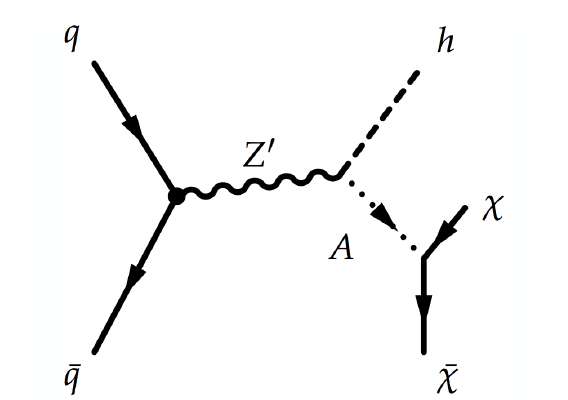
\includegraphics[width=0.5\textwidth]{img/model_fig1.png}
    \caption{The $Z'$ 2HDM model with pseudoscalar $A$}
    \label{fig:model1}
\end{figure}

%%%%%%%%%%%%%%%%%%%%%%%%%%%%%%%%%%%%%%%%%%%%%%%%%
For detector simulation, we used \texttt{Delphes 3} with latest version of delphes card used for \href{https://madanalysis.irmp.ucl.ac.be/wiki/PublicAnalysisDatabase}{CMS EXO-16-037 recasting}. The difference between custom card and default card is presented in appendix \ref{appDelphes}. We added some lines to make nertralino not to deposit energy on calorimeter. 

%The parameter changed in the \texttt{DelphesMA5tune} card was the b-tag parameter to obtain a b-tag efficiency of 70\%, as shown in \autoref{appendix:delphesma5}.

%%%%%%%%%%%%%%%%%%%%%%%%%%%%%%%%%%%%%%%%%%%%%%%%%
%%%%%%%%%%%%%%%   Cut flow  %%%%%%%%%%%%%%%%%%%%%%
%%%%%%%%%%%%%%%%%%%%%%%%%%%%%%%%%%%%%%%%%%%%%%%%%
\section{Event Selection}
There are several cuts for photon identification and background rejection. We selected only diphoton mass cut where $m_{\gamma\gamma} > 95$ GeV from diphoton with asymmetric $p_T$ threshold (30 and 18 GeV) since trigger algorithms are unknown for public. 

Next we apply cut based photon identification with loose working point for Spring 2015 (Run2) 25 ns scenario. These selection is presented in \href{https://cds.cern.ch/record/2204916?ln=en}{CMS EXO-16-011}. However, for $H/E$, we followed CMS EXO-16-012 selection, which is 0.1. Isolation is computed with $\Delta R = 0.3$.

\begin{center}
\begin{table}[h!]
	\begin{tabular}{c c c}
	\hline
	Variable & Barrel Selection & Endcap Selection\\
	\hline
	H/E& \multicolumn{2}{c}{ $< $0.1}\\
	Iso$_{ch}$ [GeV]& $<$ 3.32& $<$ 1.97\\
	$\rho$ corrected Iso$_{Neu}$ [ GeV ]& $< 1.92 + 0.14 p_T + 0.000019(p_T)^2$& $< 11.86 + 0.0139 p_T + 0.000025(p_T)^2$\\

	$\rho$ corrected Iso$_{\gamma}$ [ GeV ]& $< 0.81 + 0.0053 p_T$& $< 0.83 + 0.0034 p_T$\\
	\hline
	\end{tabular}
	\caption{Value of each variable used in barrel and endcap photon identification} \vspace*{-25pt}
\end{table}
\end{center}

In addition, two more cuts are applied to enhance the signal over background discrimination and to veto events with mismeasured $p_T^{miss}$.
\begin{itemize}
	\item $|\Delta\phi(\gamma\gamma,\,p_T^{miss})| > 2.1$
	\item $min(|\Delta\phi(jet,\,\vec p_T^{miss})|) > 0.5$ where jet reconstructed from the clustering of PF candidates
by means of the anti-kt algorithm with a distance parameter of 0.4
\end{itemize}

After these selections, we applied kinematic selections, where $p_{T_1}/m_{\gamma\gamma} > 0.5$ and $p_{T_2}/m_{\gamma\gamma} > 0.5$, for leading photon $\gamma_1$ and subleading $\gamma_2$. Moreover we imposed diphoton mass and missing transverse momentum cut, $p_{T_{\gamma\gamma}} > 90$ GeV and $p_T^{miss} > 105$ MeV.

Finally we defined signal region (SR), $120 < m_{\gamma\gamma} < 130$ GeV and $p_T^{miss} > 105$ MeV.

%%%%%%%%%%%%%%%%%%%%%%%%%%%%%%%%%%%%%%%%%%%%%%%%%
%%%%%%%%%%%%%%%   Cut flow  %%%%%%%%%%%%%%%%%%%%%%
%%%%%%%%%%%%%%%%%%%%%%%%%%%%%%%%%%%%%%%%%%%%%%%%%

\section{Cut flow}
 Unfortunately we couldn't find out detailed cutflow. Here we present the product of acceptance and efficiency for signal in the SR for each mass point only. The error is defined as $(1-(A\cdot\epsilon)^{MA5}/(A\cdot\epsilon)^{CMS})$ $(\%)$
\vskip 10pt

\begin{center}
\begin{tabular}{c c c c}
\hline
\multicolumn{4}{c}{Acceptance $\times$ efficiency $(A \cdot \epsilon)$}\\
\hline
$m_{Z_p}$ (GeV)& CMS EXO-16-012& MA5& Error\\
\hline
600& 0.317 $\pm$ 0.004& 0.317 $\pm$ 0.001& 0 \%\\
800& 0.399 $\pm$ 0.004& 0.410 $\pm$ 0.001& -2.8 \%\\
1000& 0.444 $\pm$ 0.004& 0.441 $\pm$ 0.001& 0.6 \%\\
1200& 0.474 $\pm$ 0.004& 0.343 $\pm$ 0.001& 27.6 \%\\
1400& 0.492 $\pm$ 0.004& 0.221  $\pm$ 0.001& 55.1 \%\\
1700& 0.493 $\pm$ 0.004& 0.129 $\pm$ 0.0004& 73.8 \%\\
2000& 0.351 $\pm$ 0.004& 0.082 $\pm$ 0.0002& 76.4 \%\\
2500& 0.213 $\pm$ 0.004& 0.046 $\pm$ 0.0001& 78.4 \%\\
\hline
\vspace*{20pt}
\end{tabular}
\end{center}
%%%%%%%%%%%%%%%%%%%%%%%%%%%%%%%%%%%%%%%%%%%%%%%%%
%%%%%%%   Distributions of Observables  %%%%%%%%%
%%%%%%%%%%%%%%%%%%%%%%%%%%%%%%%%%%%%%%%%%%%%%%%%%

\section{Distributions of observables}
Since missing transverse energy is important, we plotted only $ p_T^{miss}$ and $m_{\gamma\gamma}$. For this step, we made plot without normalization. For both plots from paper, the product of signal cross section and branching fraction is set to 1 fb. But we couldn't find proper values for normalization, so we presented un-normalized plots only.
\begin{figure}[h!]
\centering
\begin{minipage}{.5\textwidth}
  \centering
  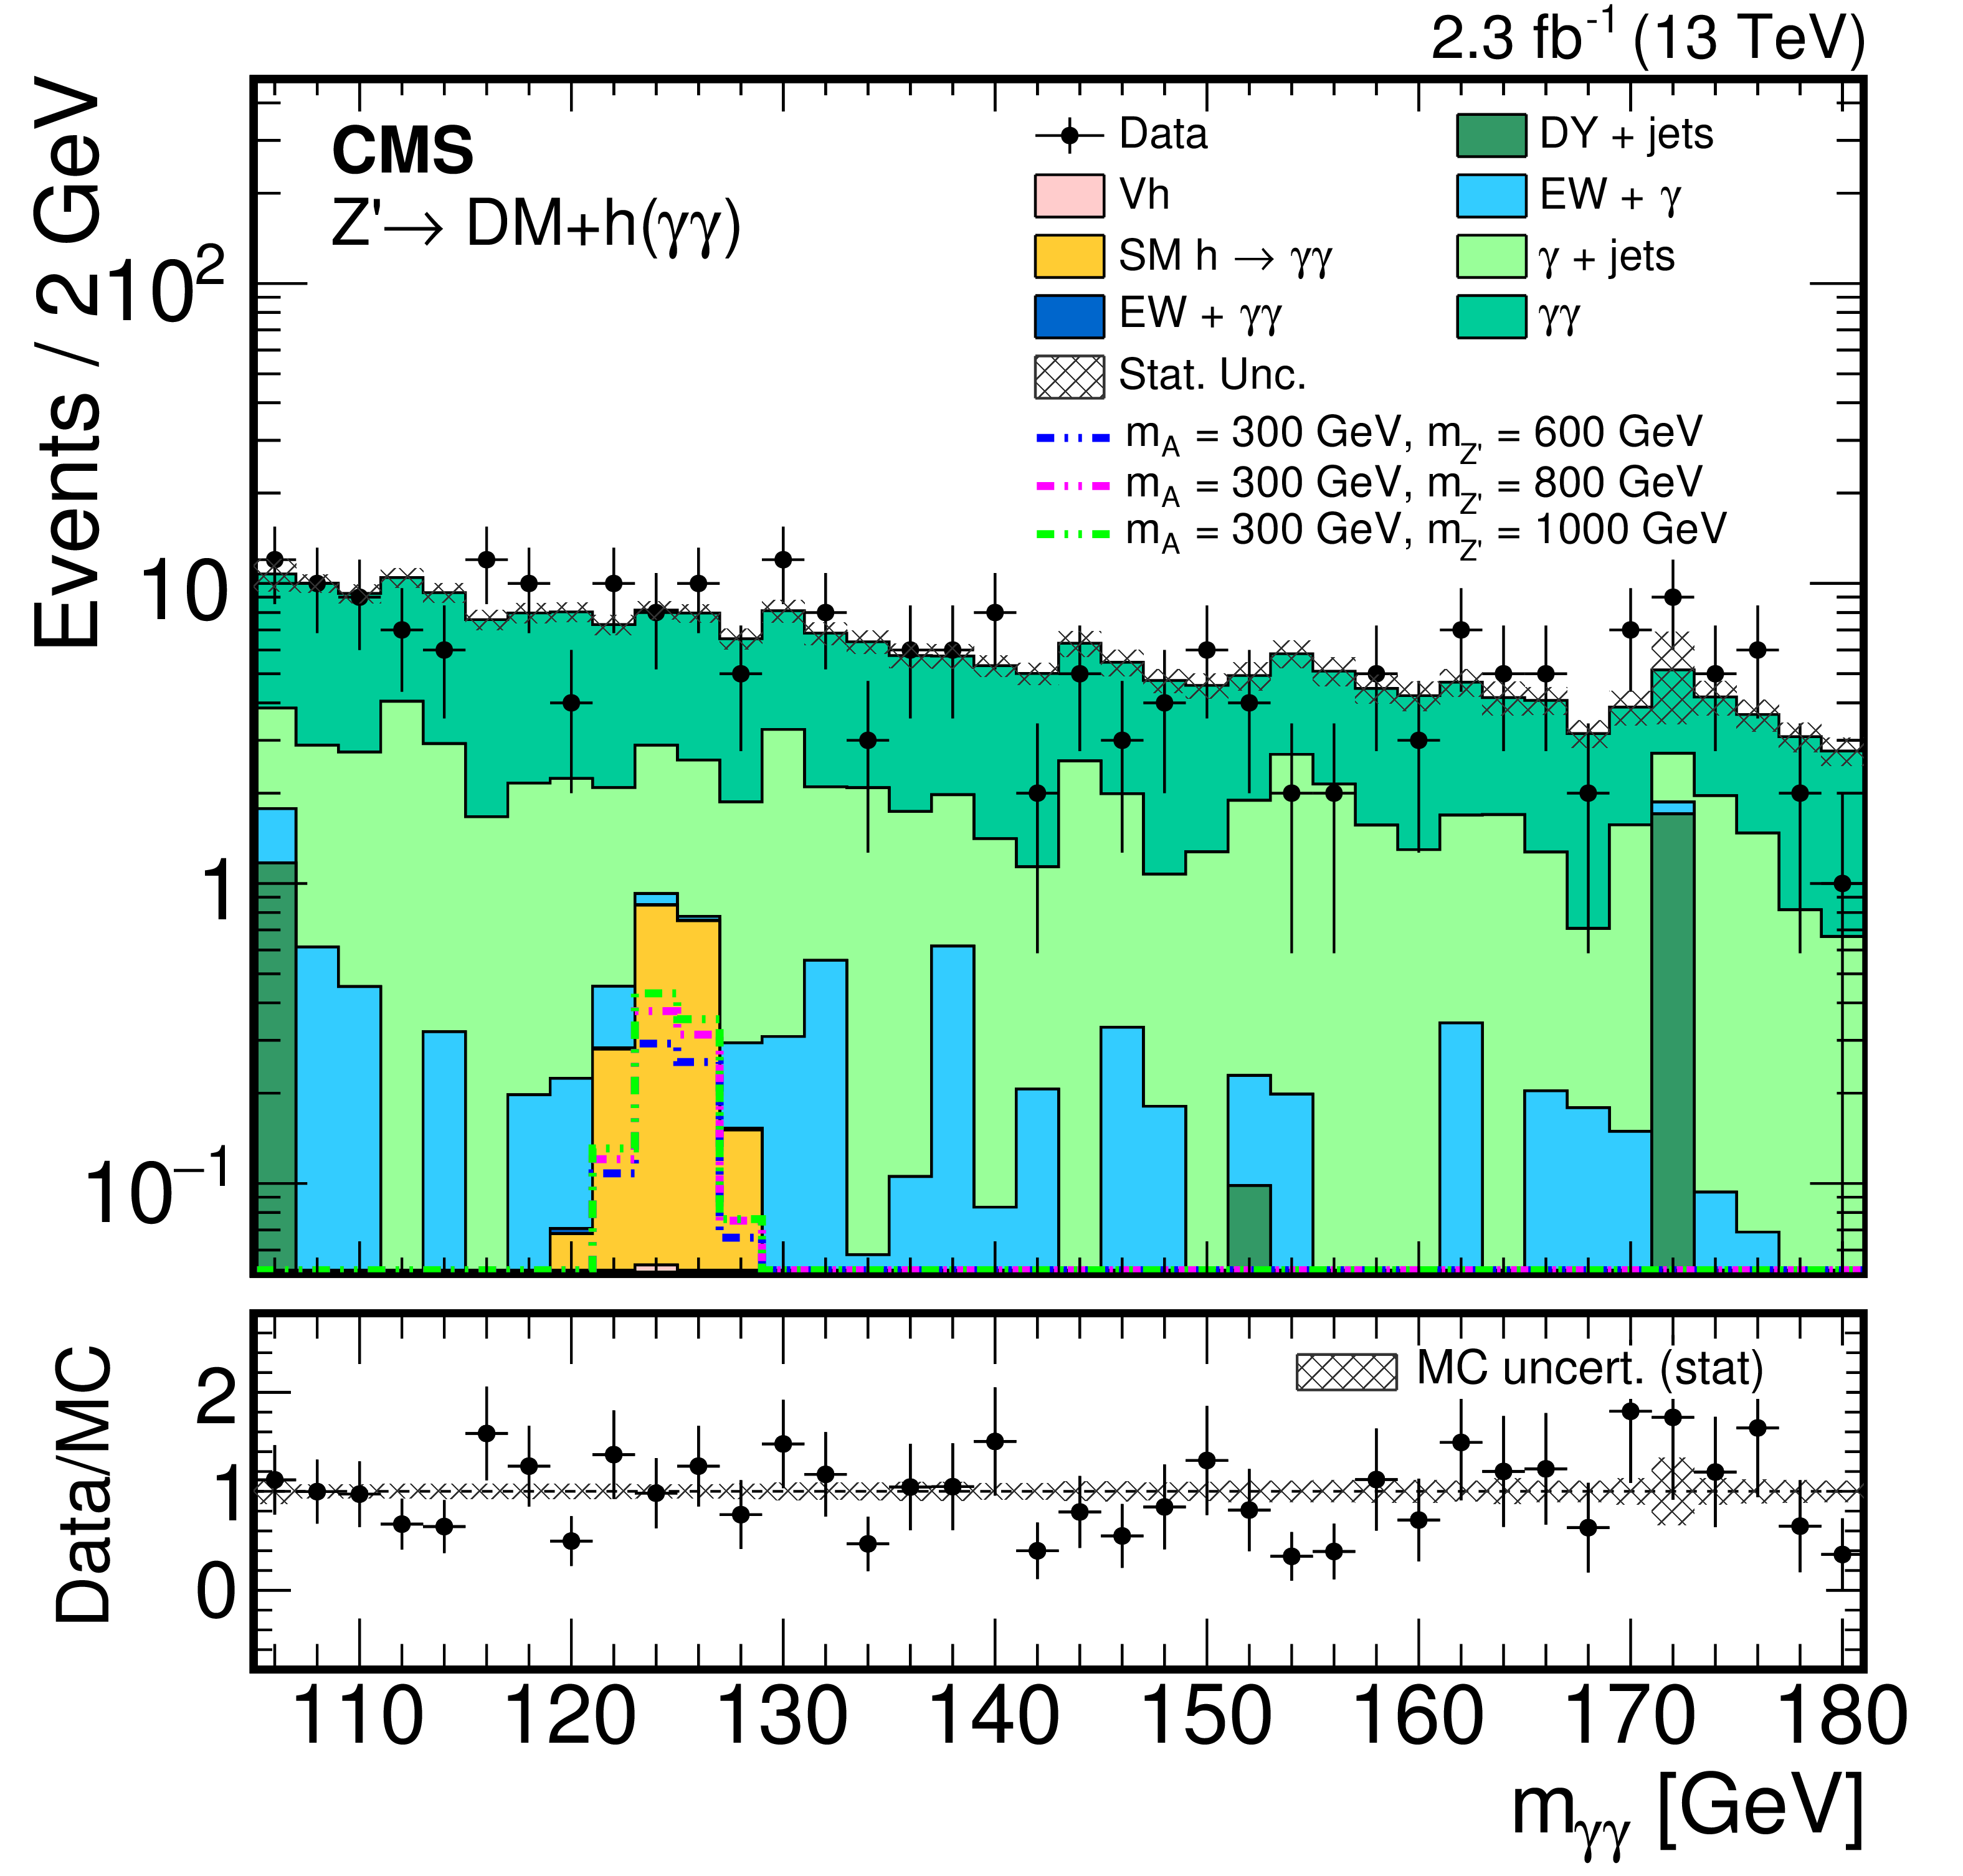
\includegraphics[scale=0.08]{img/CMS-EXO-16-012_Figure_007-a.png}
\end{minipage}%
\begin{minipage}{.5\textwidth}
  \centering
  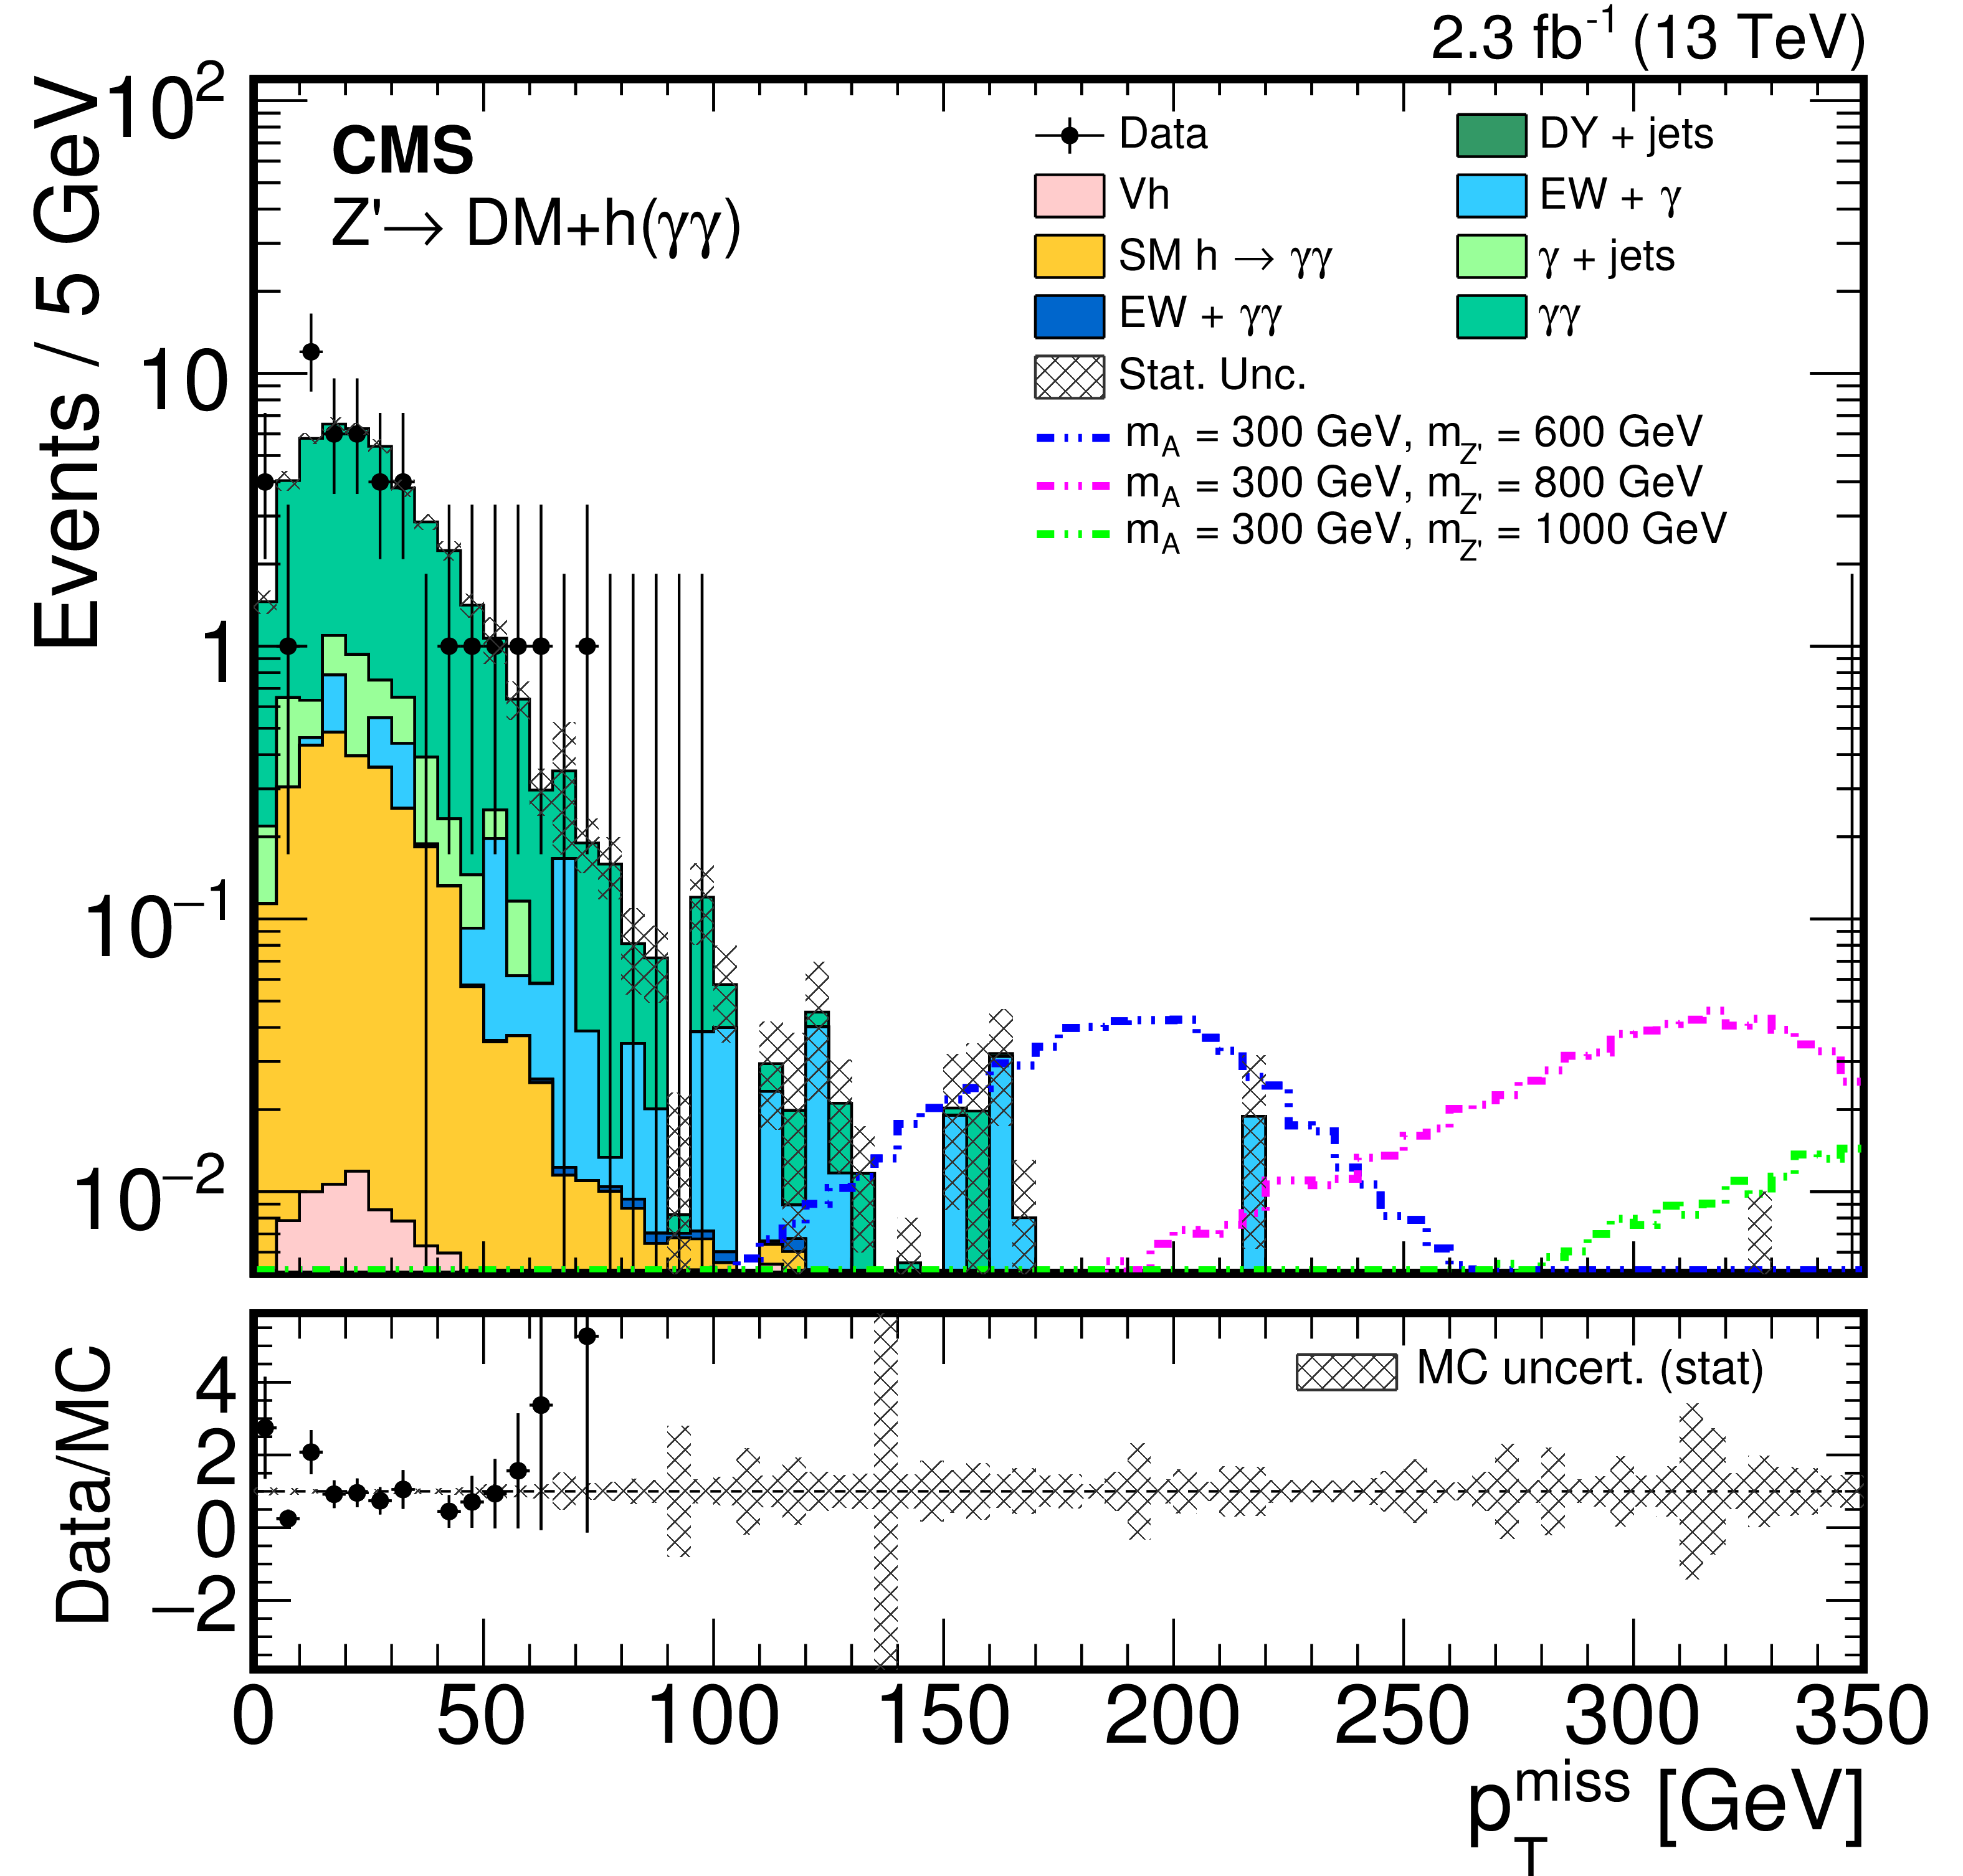
\includegraphics[scale=0.08]{img/CMS-EXO-16-012_Figure_007-b.png}
\end{minipage}
\caption{Distribution of $m_{\gamma\gamma}$ (left) in events passing all selection criteria except the $m_{\gamma\gamma}$ and $p_T^{miss}$ requirement. Distribution of $p_T^{miss}$ (right) for events passing all selection criteria including $120 \textrm{GeV} < m_{\gamma\gamma} < 130 \textrm{GeV}$ except $p_T^{miss}$ requirement. For both plots, the product of signal cross section and branching fraction is set to 1 fb.}
\end{figure}

\begin{figure}[h!]
\centering
\begin{minipage}{.5\textwidth}
  \centering
  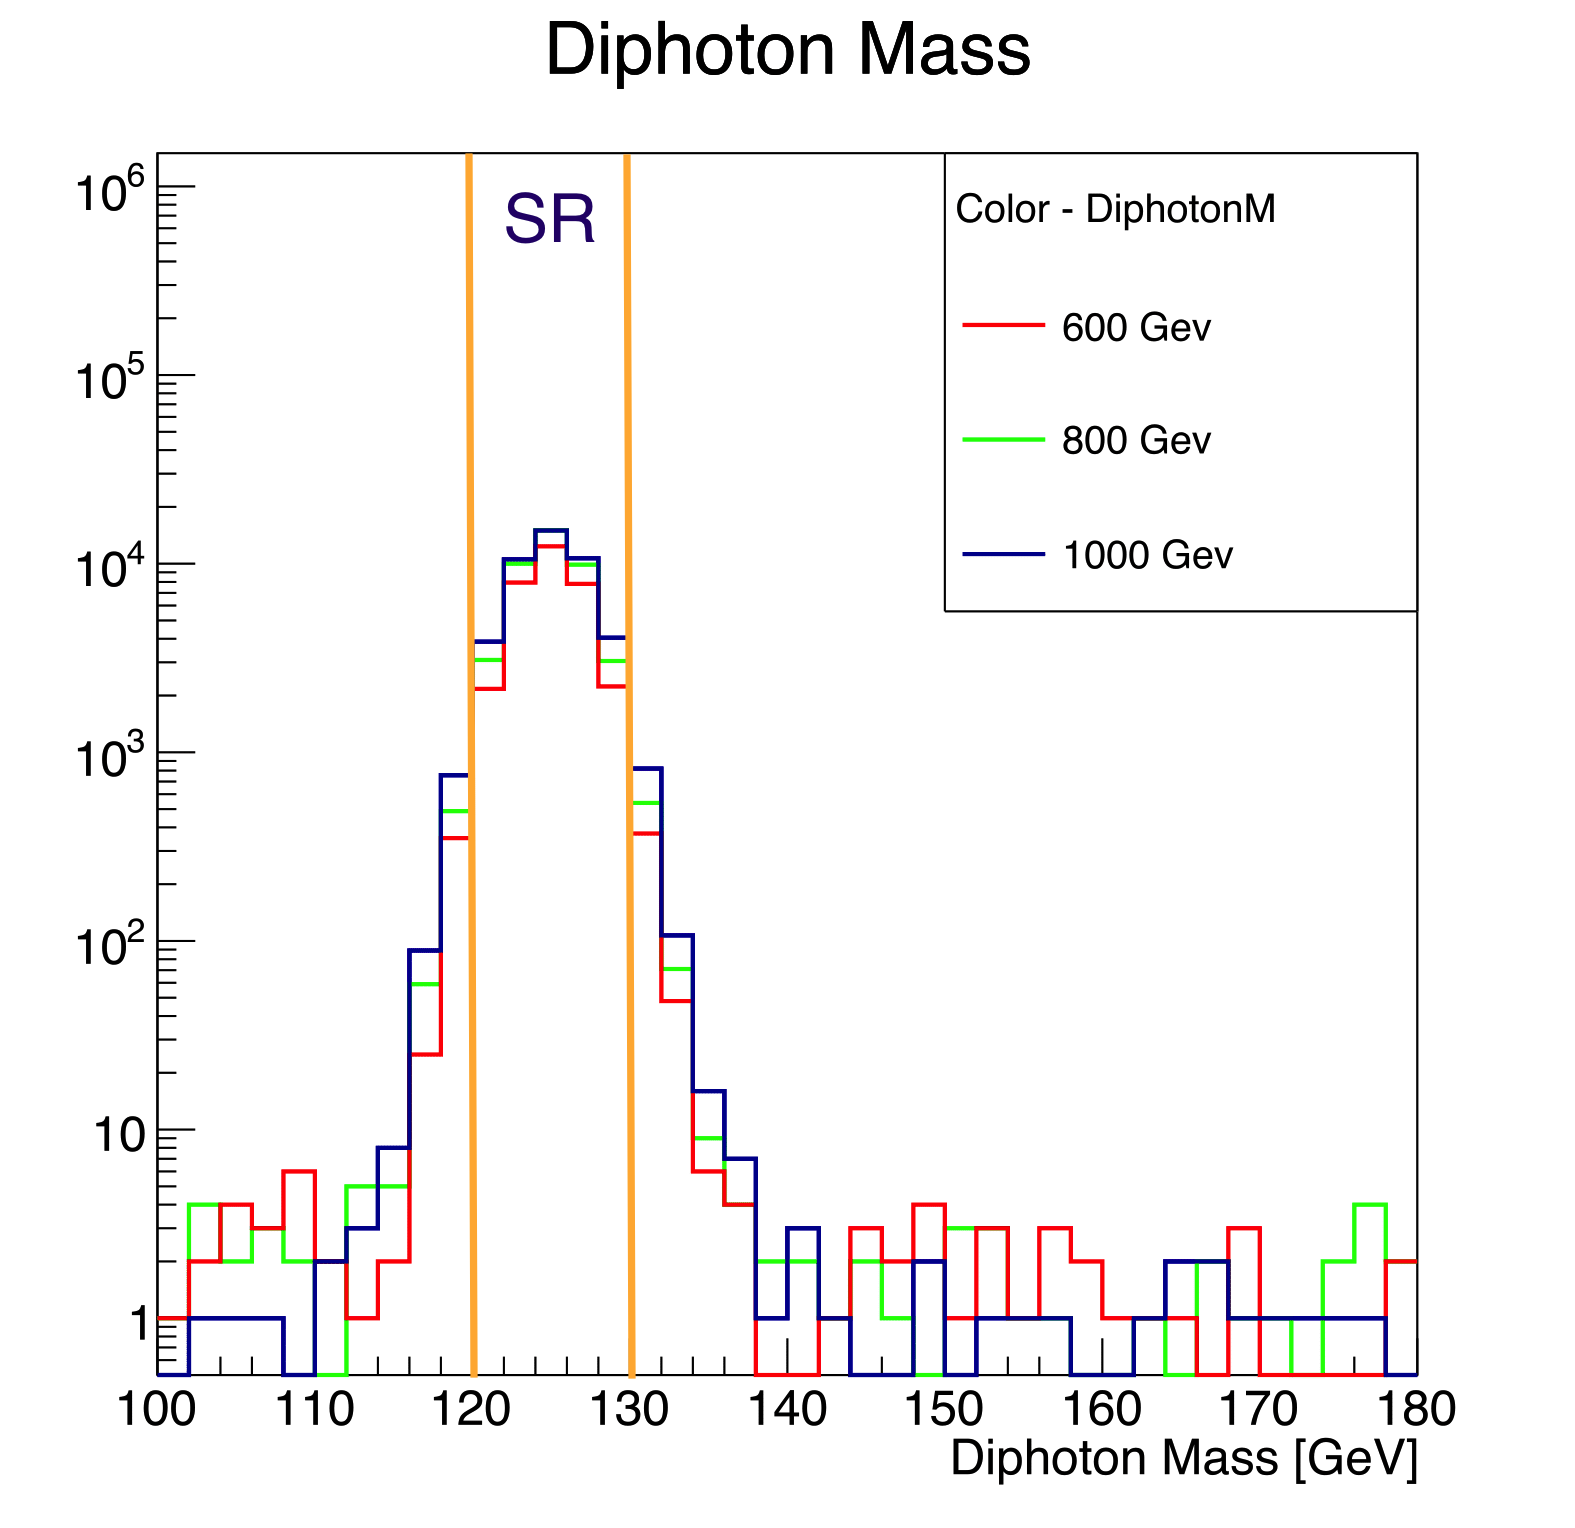
\includegraphics[scale=0.16]{img/MZp_M-1.png}
\end{minipage}%
\begin{minipage}{.5\textwidth}
  \centering
  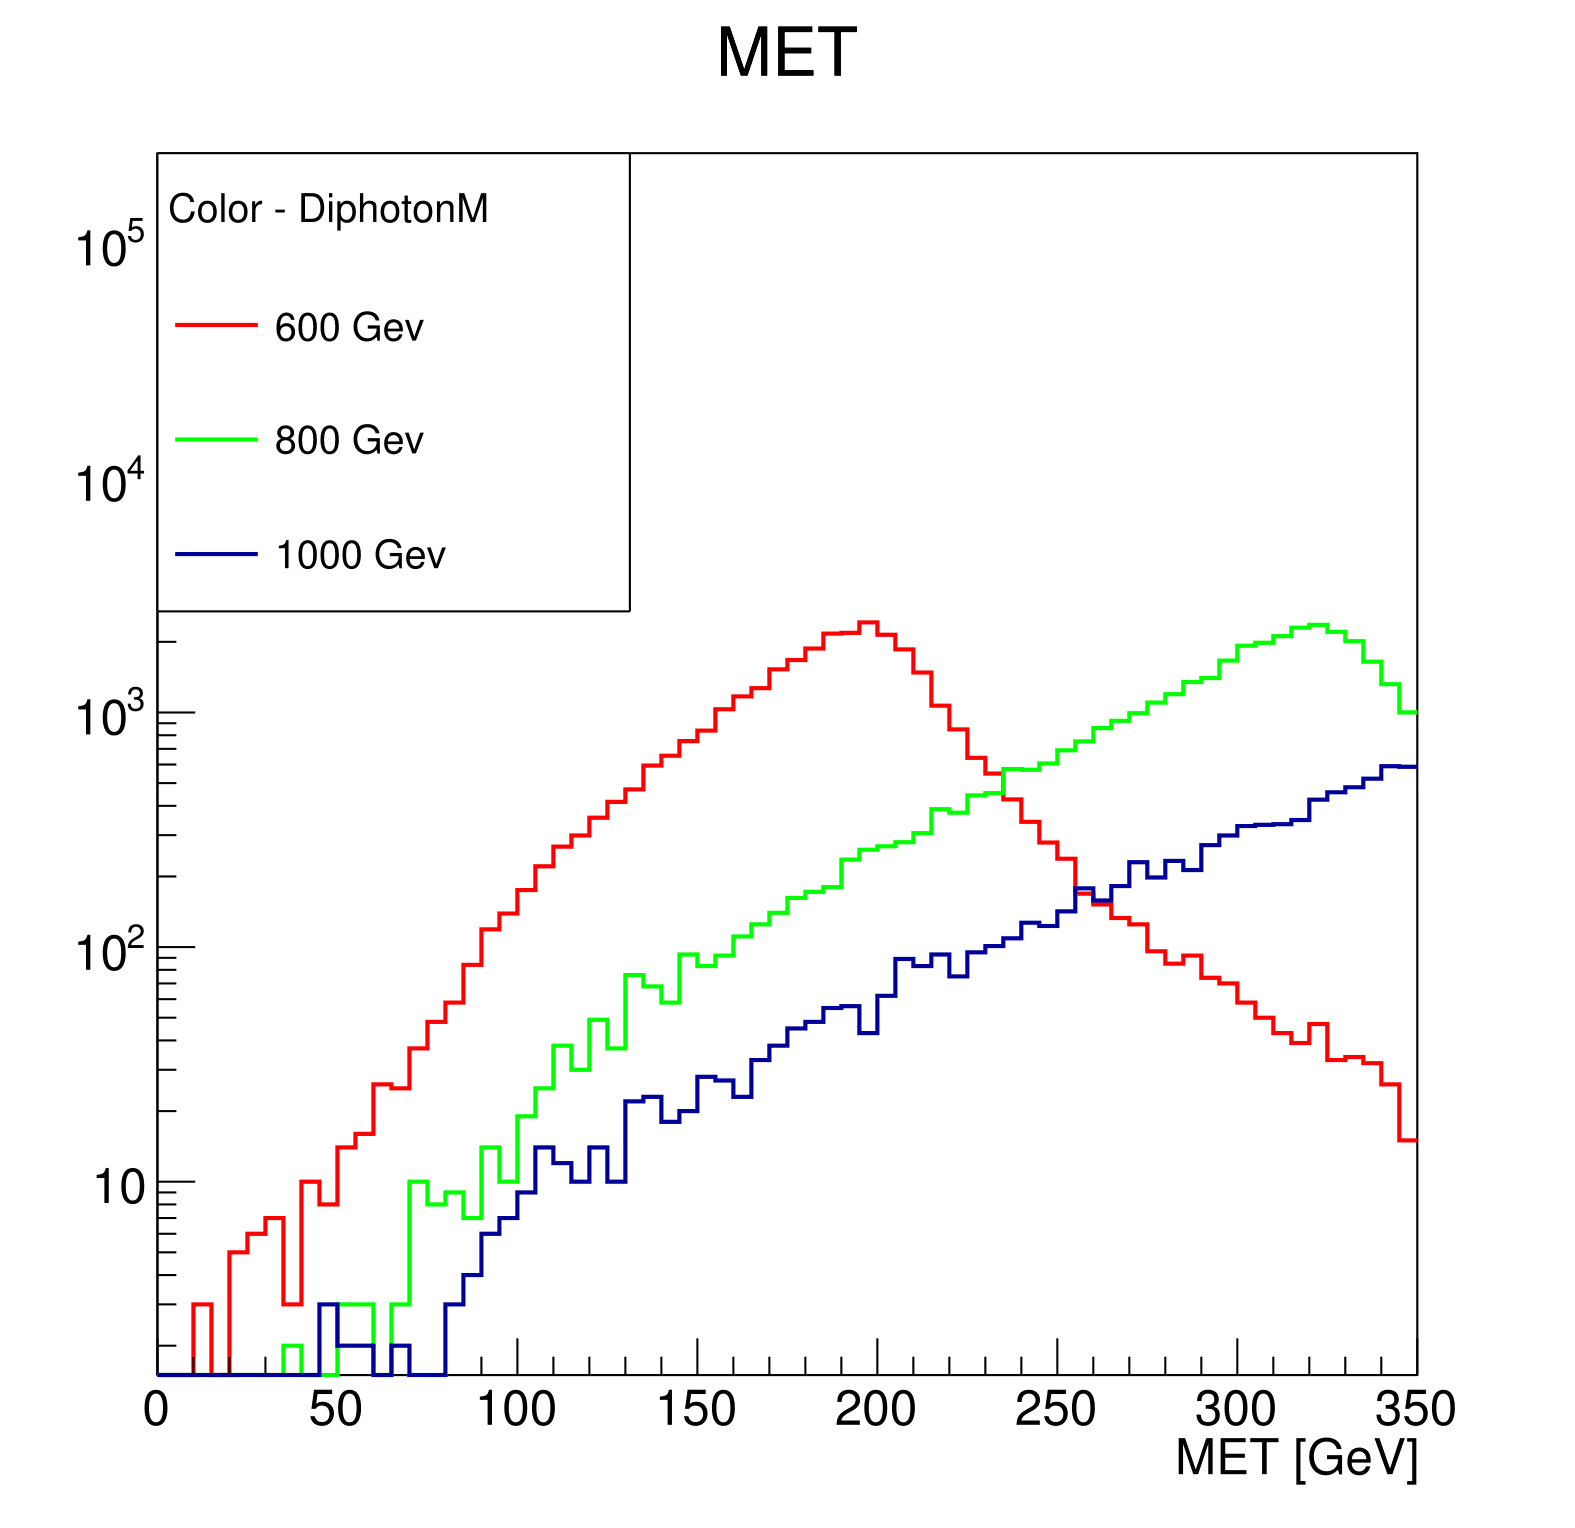
\includegraphics[scale=0.16]{img/MZp_MET-1.png}
\end{minipage}
\caption{Distribution of $m_{\gamma\gamma}$ (left) and $p_T^{miss}$ (right) with same requirement as CMS plots.}
\end{figure}

\clearpage
%%%%%%%%%%%%%%%%%%%%%%%%%%%%%%%%%%%%%%%%%%%%%%%%%
%%%%%%%%%%%%%%% Appendices %%%%%%%%%%%%%%%%%%%%%%
%%%%%%%%%%%%%%%%%%%%%%%%%%%%%%%%%%%%%%%%%%%%%%%%%

\appendix
\appendixpage
\addappheadtotoc

\section{\texttt{MadGraph MG5\_aMC} and \texttt{Pythia 8} card settings}\label{appmg5}

\lstset{language=sh}
\begin{lstlisting}

import model Zp2HDM
generate p p > Zp > h A0, A0 > n1 n1~
output Zprime_A0h_A0chichi_MZp1000_MA0300 -nojpeg

set param_card mass 32 1000
set param_card mass 26 300
set param_card mass 27 300
set param_card mass 28 300
set param_card ZpINPUTS 1 1
set param_card ZpINPUTS 2 0.8
set param_card DECAY 32 20.22504
set param_card DECAY 28 8.95228

####From the run card

 'lhapdf'  = pdlabel     ! PDF set                                     
 263400    = lhaid     ! if pdlabel=lhapdf, this is the lhapdf number
	
	
####In the shower card
!CUEP8M1 Tune
SLHA:minMassSM=1000.
SLHA:keepSM=on
SLHA:useDecayTable = off
Main:timesAllowErrors=10000
MultipartonInteractions:expPow=1.6
MultipartonInteractions:ecmPow=2.5208
MultipartonInteractions:pT0Ref=2.4024
ParticleDecays:limitTau0=on
ParticleDecays:allowPhotonRadiation=on
ParticleDecays:tau0Max=10
Check:epTolErr=1.0000000000e-02
Tune:ee=7
Tune:pp=14


!This is for decay mode
25:m0 = 125.0
25:onMode=off
25:OnIfMatch=22 22
\end{lstlisting}

\section{\texttt{Delphes} card settings}\label{appDelphes}

\lstset{language=sh}
\begin{lstlisting}
#####################
# MC truth jet finder
#####################

module FastJetFinder GenJetFinder {
  set InputArray NeutrinoFilter/filteredParticles

  set OutputArray jets

  # algorithm: 1 CDFJetClu, 2 MidPoint, 3 SIScone, 4 kt, 5 Cambridge/Aachen, 6 antikt
  set JetAlgorithm 6
  set ParameterR 0.4

  set JetPTMin 20.0
}

############
# Jet finder
############

module FastJetFinder FastJetFinder {
#  set InputArray Calorimeter/towers
  set InputArray EFlowMerger/eflow

  set OutputArray jets

  # algorithm: 1 CDFJetClu, 2 MidPoint, 3 SIScone, 4 kt, 5 Cambridge/Aachen, 6 antikt
  set JetAlgorithm 6
  set ParameterR 0.4

  set JetPTMin 20.0
}

###########
# b-tagging
###########

module BTagging BTagging {
  set JetInputArray JetEnergyScale/jets

  set BitNumber 0

  # add EfficiencyFormula {abs(PDG code)} {efficiency formula as a function of eta and pt}
  # PDG code = the highest PDG code of a quark or gluon inside DeltaR cone around jet axis
  # gluon's PDG code has the lowest priority

  add EfficiencyFormula {0} { (pt >= 30.0 && pt < 130.0) * (0.124 - 1.0*10^-3*pt + 1.06*10^-5*pt^2 - 3.18*10^-8*pt^3 + 3.13*10^-11*pt^4) +
                              (pt >= 130.0) * (0.055 + 4.53*10^-4*pt - 1.60*10^-7*pt^2) }

  add EfficiencyFormula {4} { (pt >= 30.0 && pt <205.0) * (0.40 + 1.23*10^-3*pt - 4.60*10^-6*pt^2 + 5.71*10^-9*pt^3) +
                              (pt >= 205.0) * (0.478 + 1.573*10^-4*pt)}

  add EfficiencyFormula {5} { (pt >= 30.0 && pt < 150.0) * (0.707 + 5.6*10^-3*pt - 6.27*10^-5*pt^2 + 3.10*10^-7*pt^3 - 5.63*10^-10*pt^4) +
                              (pt >= 150.0) * (0.906 - 6.39*10^-5*pt + 4.11*10^-8*pt^2) }
}

#############
#   ECAL
#############

  add EnergyFraction {18} {0.0}
  

#############
#   HCAL
#############

  add EnergyFraction {18} {0.0}

\end{lstlisting}


\end{document}
